\documentclass{article}

% Import custom style file containing common packages and options
\usepackage{preamble}
\addbibresource{./references.bib}
\graphicspath{{./Figures/}}

% Discrete Fourier Transform
\newcommand{\GenP}{\hat{P}_m}
\newcommand{\POne}{\hat{P}_1}
\newcommand{\PTwo}{\hat{P}_2}
\newcommand{\PThree}{\hat{P}_3}
\newcommand{\PFour}{\hat{P}_4}

% Continuous Fourier Transform
\newcommand{\GenPk}{\hat{P}(\kappa)}
\newcommand{\PZerok}{\hat{P}(0)}

% Define custom math symbols
\DeclareMathOperator{\cn}{Cn}
\DeclareMathOperator{\sgn}{sgn}
\DeclareMathOperator{\Ur}{Ur}
\DeclareMathOperator{\Sk}{Sk}
\DeclareMathOperator{\As}{As}
\DeclareMathOperator{\Bi}{Bi}

% Define \im as Roman i
\newcommand{\im}{\mathrm{i}}
% Replace epsilon with varepsilon
\renewcommand*{\epsilon}{\varepsilon}

% Use \thalf and \squart commands from JFM class
\newcommand\squart{\ensuremath{{\textstyle\frac{1}{4}}}}
\newcommand\thalf{\ensuremath{{\textstyle\frac{1}{2}}}}

\linenumbers

\title{Wind-Induced Changes to Surface Gravity Wave Shape in Shallow Water}

\author{Thomas J. Zdyrsk \and Falk Feddersen}

\begin{document}

\maketitle

\begin{abstract}
Wave shape (e.g.,\ wave skewness and asymmetry) impacts sediment
transport, beach morphology, and ship safety.
Previous work by the authors showed that wind (via changes in surface
pressure) affects wave shape in intermediate and deep water.
This effect was most pronounced as the depth ($kh$) decreased.
Here, this work investigates the interaction of wind and wave shape in
shallow water.
A multiple-scales analysis is applied to waves propagating over a
shallow ($kh \ll 1$), flat bottom with a variety of wind-induced
surface-pressure profiles, such as Jeffreys-type and generalized
Miles-type.
The shallow depth enhances the influence of wind on wave shape and
intensifies the waves' second-harmonic modes.
The results are compared to previous wave-tank experimental data and
numerical simulation results.
\end{abstract}

\section{Introduction}
Directly comparing with \textcite{feddersen2005wind} may be challenging
though; that experiment generated monochromtic, sinusoidal waves that
were subsequently forced by the wind.
However, since sinusoidal waves are not eigenfunctions of the KdV
equation, they will evolve (namely, energy will be passed to higher
harmonics even in the absence of wind).
Indeed, such a phenomena---in the unforced case---was observed over a
flat bottom by \textcite{chen2004incorporation}, where the primary and
first harmonic traded energy back and forth periodically.
This same setup was treated numerically by \textcite{liu2016modeling}
who also included the effects of wind.
The growth/decay of waves by wind was superimposed on this oscillation
amongst modes.

\Textcite{liu2016modeling} also claim that this harmonic-oscillation
means that some downwind locations will measure virtually no skewness
or asymmetry, while others will.
They claim that this explains the observations of
\textcite{feddersen2005wind}: the flat-bottomed portion of the tank saw
minimal effect of wind speed on skewness/asymmetry since it was located
at a node of this harmonic oscillation.
However, a wind-speed dependent change was observed on the sloping beach
portion since this measurement location was not a node.
Note that this argument does not apply to the (pseudo-shallow water)
experiments by \textcite{leykin1995asymmetry}: these waves were not
mechanically generated, but rather purely wind-generated.
Therefore, they do not necessarily begin as pure sinusoids and hence do
not suffer from these harmonic oscillations (likely being closer to
cnoidal waves, which do not experience such oscillations).

\section{Problem Solving Technique}
The governing equations are%
\footnote{
  We used the gauge freedom to absorb the Bernoulli ``constant'' $C(t)$
  in the dynamic boundary condition into the definition of $\phi$.
}
\begin{alignat}{2}
  0 &= \phi_{xx} + \phi_{yy} + \phi_{zz} &&\qq{on}
  -h < z < \eta \,, \label{eq:laplace}\\
  0 &= \phi_{z} &&\qq{on} z=-h \,, \label{eq:bottom_bc}\\
  \phi_{z} &= \eta_{t} + \phi_{x} \eta_{x} +
  \phi_{y} \eta_{y} &&\qq{on} z = \eta \,, \label{eq:kinematic_bc}\\
  \qq*{and} 0 &= \frac{p}{\rho_w} + g\eta + \phi_{t} +
  \frac{1}{2} \bqty{\phi_{x}^2 + \phi_{y}^2 + \phi_{z}^2} &&\qq{on} z=
  \eta \,. \label{eq:dynamic_bc}
\end{alignat}
We are seeking a quasi-periodic progressive wave of permanent form:
\begin{gather}
  \eta(\vec{x},t) = \eta(\theta, t) \qq{with} \theta \coloneqq
  \vec{x}\vdot\vec{k} - \omega t \,, \\
  \eta(\theta + 2\pi,t) = \eta(\theta,t) \,,
  \label{eq:periodicity_condition}
\end{gather}
with similar conditions on $\vec{u} \coloneqq \grad{\phi}$.
We are parameterizing our wave by four quantities: the depth, mean
Eulerian current, wave height, and wavelength.
We will use Stokes' first definition of wave celerity by taking the mean
current to be zero:
\begin{equation}
  \bar{u} = 0. \label{eq:celerity_definition}
\end{equation}
Additionally, we will choose our $z$-datum at the mean water level so that
$\overline{\eta}$ vanishes.
Finally, we assume the surface pressure $p(x,t)$ can be expressed as a
convolution of some (time-independent) function with $\eta(x,t)$:
\begin{equation}
  p(x,t) = \mathcal{P}(x) \star \eta(x,t) \implies \hat{p}_m = k \GenP
    \hat{\eta}_m \,,
\end{equation}
with $\hat{g}_m$ the Fourier transform of a function $g(x,t) =
\Re{\sum_{m=0}^{\infty} \hat{g}_m \exp(\im m x)}$.
Here, $\GenP \in \mathbb{C}$ is an arbitrary coefficient; some select
values are
$\GenP = m P_J e^{\im \psi_P}$ and $\psi_P = \pm \thalf \pi$
for Jeffreys, $\GenP = P_M \exp(\im \sgn{m} \psi_P)$ for Miles, and
$\GenP = P_G \exp(\im m \psi_P)$ for Generalized Miles surface pressure
profiles.
Note, the wind phase $\psi_P$ is a free parameter for the Miles and
Generalized Miles profiles.

\section{Normalization}
We will normalize by identifying characteristic scales.
The parameters we know \apriori are the wavenumber $k$, the wave
amplitude $a$ (to be clarified later), the depth $h$, $g$, and the
wind speed $U$ expressed as a pressure magnitude $P \propto \rho_a U^2$.
Denoting nondimensional variables with an accent, we have
\begin{equation*}
  \begin{aligned}
  x &= \frac{x'}{k} \,, \\
  y &= \frac{y'}{k} \,, \\
  z &= h z' \,,
  \end{aligned}
  \qquad
  \begin{aligned}
  t &= \frac{t'}{k\sqrt{g h}} \,, \\
  \eta &= a \eta' \,, \\
  \phi &= \phi'\frac{a}{k}\sqrt{\frac{g}{h}} \,,
  \end{aligned}
  \qquad
  \begin{aligned}
  p &= \alpha p' \rho_w g a \,, \\
  P &= \alpha P' \frac{\rho_w g}{k} \,.
  \end{aligned}
\end{equation*}
Here, we have defined a parameter $\alpha \coloneqq \order{P k/(\rho_w g
)}$.
Using these definitions, our equations take the form
\begin{alignat}{2}
  0 &= \mu \pqty{\phi'_{x'x'} + \phi'_{y'y'}} + \phi'_{z'z'} &&\qq{on}
    -h' < z' < \epsilon \mu \eta' \,, \label{eq:laplace_nondim} \\
  0 &= \phi'_{z'} &&\qq{on} z'=-h' \,, \label{eq:bottom_bc_nondim} \\
  \phi'_{z'} &= \mu \eta'_{t'} +
    \epsilon \mu \bqty{\phi'_{x'} \eta'_{x'} + \phi'_{y'} \eta'_{y'}}
    &&\qq{on} z' = \epsilon \eta' \,, \label{eq:kinematic_bc_nondim} \\
  0 &= \alpha p' +  \eta' + \phi'_{t'} + \frac{1}{2}
    \bqty{\epsilon \pqty{\phi_{x'}^{\prime \, 2} + \phi_{y'}^{\prime \,
    2}} +  \frac{\epsilon}{\mu} \phi_{z'}^{\prime \, 2}} &&\qq{on} z'=
    \epsilon \eta' \,.  \label{eq:dynamic_bc_nondim}
\end{alignat}
The primes will be dropped henceforth for readability.
Here, we chose, $\alpha = P k/(\rho_w g)$, $\mu = (k h)^2$ and
$\epsilon = a / h$.
Furthermore, we see that $\epsilon/\mu$ is (up to some numerical
prefactors) the Ursell number, $\Ur = H \lambda^2/d^3$.

Now, we will estimate the wind speeds associated with different pressure
magnitudes $P$.
For the deep water case, we related $P$ to the wind-induced energy growth
rate $\gamma$, which was then be related to the friction velocity $u_*$
through experimental measurements, which was finally converted to
$U_{10}$ wind speeds using logarithmic boundary layer theory.
Here, we encounter an issue: the experimental measurements are taken for
deep water, and are not necessarily expected to hold for shallow water
waves.

We will use the \textcite{miles1957generation} theory for $P' \ll 1$ as a model%
\footnote{
  Though Miles does specialize to deep-water waves partway through the
  derivation, the equation we utilize is applicable to both shallow and
  deep water.
  The only difference is that $m = \rho_w/k$ and $s=\rho_a/\rho_w$,
  which Miles uses for deep water, should be replaced by
  $m=\rho_w\coth(kh)/k$ and $s = \tanh(kh) \rho_a/\rho_w$.
  Hence, the extra factor of $\tanh(kh)$ appearing in
  \cref{eq:miles_growth_rate}.
}%
, where
\begin{equation}
  p_M = k \rho_a U^2 \Re{(\tilde{\alpha} + \im \tilde{\beta}) \eta_a}
  \coloneqq k P_M \Re{ e^{\im \psi_P} \eta_a} \,.
\end{equation}
with $U$ a characteristic wind speed and $\eta_a$ the analytic
representation%
\footnote{
  The analytic representation of a real function $f(x)$ is $f(x) + \im
  \hat{f}(x)$ with $\hat{f}(x)$ the Hilbert transform of $f(x)$.
  For our purposes, only two representations will be relevant: the
  analytic representation of $\cos(x)$ is $e^{\im x}$ and that of
  $\sin(x)$ is $-\im e^{\im x}$.
}
of $\eta$.
This gives a relationship between the pressure magnitude $P$ and growth
rate $\gamma$ as
\begin{equation}
  \frac{\gamma}{\omega_0} \approx \frac{\gamma}{\Re{\omega}} \coloneqq
  \frac{1}{\omega E} \pdv{E}{t}
  = \tilde{\beta} \frac{\rho_a}{\rho_w} \frac{U^2}{c_0^2} \tanh(kh)
  = \tilde{\beta} \frac{\rho_a}{\rho_w} \frac{U^2 k}{g} \,,
  \label{eq:miles_growth_rate}
\end{equation}
with $c_0 = \sqrt{g\tanh(kh)/k}$ and $\omega_0 = c_0 k$.
Using our definition for $P_M \exp(\im \psi_P) = (\tilde{\alpha} + \im
\tilde{\beta}) \rho_a U^2$, we find
\begin{equation}
  \frac{\gamma}{\omega_0} \approx \frac{P_M k}{\rho_w g} \sin(\psi_P)
  = P'_M \alpha \sin(\psi_P)
  ,
\end{equation}
Note that this also matches the $P = \order{\epsilon}$ growth rate we
derive for the Jeffreys case (\ie $\psi_P = \pm \pi/2$) in
\cref{sec:energy_growth_rate}.

According to \textcite{donelan2006wave}, the wind speed and growth rate
are related in shallow water by
\[
  \frac{\gamma}{\omega_0} = \frac{\rho_a}{\rho_w} (ak)
  \pqty{\frac{U_{\lambda/2}}{c_0} - 1}^2
  G \bqty{(ak)
  \pqty{\frac{U_{\lambda/2}}{c_0} - 1}^2}
\]
with $G[x] = b - q \mathcal{H}(x - 1)$ with $b = 4.91$, $q = 3.98$, and
$\mathcal{H}$ the Heaviside unit step function.
Finally, in the logarithmic boundary layer, we have
\[
  \frac{U_z}{\ln(z/z_0)} = \text{const}
  \implies U_{z} = U_{\lambda/2} \frac{\ln(z/z_0)}{\ln[\lambda/(2 z_0)]}
\]
with \autocite{taylor2001dependence}
\[
  \frac{z_0}{H} = 1200 \pqty{\frac{H}{\lambda}}^{4.5}
\]
where $H$ is the wave height.
Combining this, we find
\[
  P'_M \alpha = \frac{\rho_a}{\rho_w} \csc(\psi_P)
  y \Bqty{b-qH[y - 1]} \qq{with}
  y \coloneqq
  \epsilon \sqrt{\mu}
  \pqty{\frac{U_{z}}{c_0} \frac{\ln(2400)+5.5\ln(\epsilon \sqrt{\mu}/\pi)}
    {\ln(1200) + 4.5 \ln(\epsilon \sqrt{\mu}/\pi) + \ln(H/z)} - 1}^2
\]
with $T$ the wave period.
If we take $\psi_P = 3\pi/4$ and $\rho_a/\rho_w = \num{1.225e3}$, we get
\[
  P'_M \alpha = \num{1.7e-3} y \Bqty{b-q \mathcal{H}[y - 1]}
\]
with $y$ given above.

If we take $\mu = \epsilon = 0.1$, $\rho_a/\rho_w = 10^{-3}$, $T =
\SI{10}{\second}$, $h = \SI{10}{\meter}$, and $z = \SI{10}{\meter}$, we
find
\[
  y = \num{3.2e-2} \pqty{U_{10} \SI{0.12}{\second\per\meter} - 1}^2
\]
For $U_{10} < \SI{56}{\meter\per\second}$, we have
\[
  P'_M \alpha = \SI{3.8e-6}{\second\squared\per\meter\squared} U_{10}^2
\]
For instance, $U_{10} = \SI{50}{\meter\per\second}$ gives
$P'_M \alpha = \num{6.5e-3} \approx \epsilon^2$.

If we instead consider laboratory conditions with $h=\SI{0.23}{\meter}$,
$kh = 0.85$, and $a/h = 0.25$ as in \textcite{feddersen2005wind}, we
instead get
\[
  y = \num{0.21} \pqty{U_{10} \SI{0.87}{\second\per\meter} - 1}^2
\]
For $U_{10} > \SI{3.7}{\meter\per\second}$, we have
\[
  P'_M \alpha = \SI{2.6e-4}{\second\squared\per\meter\squared} U_{10}^2
\]
For instance, $U_{0.3} = \SI{8}{\meter\per\second}$ gives
$P'_M \alpha = \num{1.2e-2} \approx \epsilon^3$.

\section{Depth Dependence of \texorpdfstring{$\phi$}{Velocity Potential}}
First, we will determine the depth dependence of $\phi$ implied by
Laplace's equation.
We will do this be expanding $\phi$ in a Taylor series about the bottom
$z=-1$:
\begin{equation}
  \phi(x,y,z,t) = \sum_{n=0}^\infty (z+1)^n\phi_n(x,y,t) \,.
\end{equation}
Derivatives in the $\vu{z}$ direction give
\begin{equation}
  \pdv[2]{\phi}{z} = \sum_{n=2}^{\infty} (n-1)(n)(z+1)^{n-2}\phi_n =
  \sum_{n=0}^{\infty} (n+1)(n+2)(z+1)^n\phi_{n+2} \,.
\end{equation}
Denoting the horizontal gradient as $\grad_X \coloneqq
(\pdv{x},\pdv{y})$,
Laplace's equation, \cref{eq:laplace_nondim}, gives
\begin{equation}
  \mu \laplacian_X{\phi} + \pdv[2]{z} \phi = \sum_{n=0}^\infty
  (z+1)^n\pqty{\mu \laplacian_X \phi_n + (n+1)(n+2)\phi_{n+2}} = 0 \,.
\end{equation}
Since this holds for arbitrary $z \in [-1,\epsilon \eta]$, each
term in the series must vanish, giving a recursion relation:
\begin{equation}
  \phi_{n+2} = \frac{-\mu \laplacian_X{\phi_n}}{(n+1)(n+2)} \,.
\end{equation}

We assumed previously that we were dealing with a horizontal
bottom-boundary.
Then, our bottom-boundary condition, \cref{eq:bottom_bc_nondim}, implies
\begin{equation}
  \pdv{\phi}{z}\eval_{z=-1} = \pqty{\sum_{n=1}^\infty
  n(z+1)^{n-1}\phi_n}\eval_{z=-1} = \phi_1 = 0 \,.
\end{equation}
Therefore, the recursion relation shows that $\phi_n=0$ for all odd $n$.
Hence, we've found a partial expansion of $\phi$ in terms of $\mu$:
\begin{equation}
  \phi(x,y,z,t) = \sum_{n=0}^{\infty} (-\mu)^n \frac{(z+1)^{2n}}{(2n)!}
  \grad_{X}^{2n} \phi_0(x,y,t; \mu, \epsilon) \,.
  \label{eq:phi_expansion}
\end{equation}
If we assume $\mu \ll 1$, we have,
\begin{equation}
  \phi = \phi_0 - \frac{1}{2}\mu (z+1)^2\laplacian_X\phi_0 +
  \frac{\mu^2}{24}(z+1)^4\laplacian_X\laplacian_X\phi_0 +
  \order{\mu^3} \,.
\end{equation}

Using \cref{eq:laplace_nondim,eq:bottom_bc_nondim}, we have determined
the depth dependence of $\phi$.
Therefore, our remaining goal is to determine the form of $\eta$ and
$\phi_0$.
For convienence, we will define $\varphi \coloneqq \phi_0$, as we will
need to append more subscripts shortly.

Note that truncating our series $\phi_n$ at finite $n$ means
Laplace's equation is only satisfied approximately.
This is in contrast to the intermediate-depth water case, where we were
able to satisfy Laplace's equation identically at each order.

Substituting this series expansion into the two
remaining boundary equations,
\cref{eq:kinematic_bc_nondim,eq:dynamic_bc_nondim}, we have reduced our
system of equations to
\begin{gather}
  \eta_t + \grad_X{H}\vdot\pqty{\grad_X\varphi
    -\frac{1}{2}\mu H^2\laplacian_X\grad_X\varphi} =
    -H\laplacian_X\varphi
  +\frac{1}{6}\mu H^3\laplacian_X\laplacian_X\varphi +
    \order{\mu^2}, \\
  p + \eta + \varphi_{t} - \frac{1}{2}\mu H^2\laplacian_X\varphi_{t} +
    \frac{1}{2}\epsilon \pqty{\grad_X\varphi}^2 = \order{\mu^2}
    \,.
\end{gather}
Note that we have used the total depth $H\coloneqq 1+\epsilon\eta$.
These equations can be simplified slightly to give
\begin{gather}
  \eta_t + \grad_X(H\grad_X\varphi)
    -\frac{1}{6}\mu \grad_X\vdot(H^3\laplacian_X\grad_X\varphi) =
    \order{\mu^2} \,, \\
  p + \eta + \varphi_{t} - \frac{1}{2}\mu H^2\laplacian_X\varphi_{t} +
    \frac{1}{2}\epsilon\pqty{\grad_X\varphi}^2 = \order{\mu^2}
    \,.
\end{gather}

\subsection{Restrictions}
At this point, we will again restrict our attention to one-dimensional
waves:
\begin{gather}
  \eta_t + \pqty{H\varphi_x}_x
    -\frac{1}{6}\mu \pqty{H^3\varphi_{xxx}}_x =
    \order{\mu^2}, \label{eq:kinematic_bc_varphi} \,, \\
  \eta + \varphi_t - \frac{1}{2}\mu H^2\varphi_{txx} +
    \frac{1}{2}\epsilon\pqty{\varphi_x}^2 = \order{\mu^2} \,.
  \label{eq:dynamic_bc_varphi}
\end{gather}
Further, we will now assume $\epsilon = \mu \ll 1$ which implies $\Ur
\approx 1$.

\section{Perturbation Expansion}
\label{sec:shallow_water}
We expand our timescale in terms of multiple timescales $t_n =
\epsilon^n t$ for $n= 0,1,2,\ldots$.
Thus, all time derivative become $\partial_t \to \partial_{t_0} +
\epsilon \partial_{t_1} + \ldots$.
Then, we expand our variables in an asymptotic series of $\mu$
\begin{align}
  \eta(x,t) &= \sum_{k=0}^{\infty} \epsilon^k
    \eta_{k+1}(x,t_0,t_1,\ldots) \,, \\
  \varphi(x,t) &= \sum_{k=0}^{\infty} \epsilon^k
    \varphi_{k+1}(x,t_0,t_1,\ldots) \,, \\
  p(x,t) &= \sum_{k=0}^{\infty} \epsilon^k p_{k+1}(x,t_0,t_1,\ldots)
    \,.
\end{align}

\section{\label{sec:intermediate} \texorpdfstring{Intermediate Wind:
$\alpha = \epsilon$}{Intermediate Wind}}
Here, we assume $\alpha \coloneqq P k/(\rho_w g) = \epsilon$.
\subsection{Zeroth Order Equations}
Collecting order-one terms $\order{\epsilon^0}$ from
\cref{eq:kinematic_bc_varphi,eq:dynamic_bc_varphi} gives
\begin{gather}
  \pdv{\eta_0}{t_0} + \pdv[2]{\varphi_0}{x} = 0 \,, \\
  \eta_0 + \pdv{\varphi_0}{t_0} = 0 \,.
\end{gather}
Eliminating $\eta_1$ from this gives
\begin{equation}
  \pqty{\pdv[2]{t_0} - \pdv[2]{x} } \varphi_0 = 0 \,.
  \label{eq:wave_eq}
\end{equation}
This is the standard one-dimensional wave equation.
This implies
\begin{equation}
  \varphi_0 = f_0(x-t_0,t_1) + g_0(x+t_0,t_1) \,.
  \label{eq:phi0_sol}
\end{equation}
We will restrict to right-moving waves and take $g_0 = 0$.
This also gives
\begin{equation}
  \eta_0 = - \pdv{\varphi_0}{t_0} = f_0'(x-t_0,t_1) \,,
  \label{eq:eta0_sol}
\end{equation}
with $f_0'(x-t_0,t_1) \coloneqq \eval{\pdv*{\theta}
f_0(\theta,t_1)}_{\theta = x-t_0}$.

\subsection{\label{sec:int_first_order} First Order Equations}
Continuing to the next order of perturbation theory, we retain terms of
order $\order{\epsilon}$.
Inserting our previous solutions, \cref{eq:phi0_sol,eq:eta0_sol} yields
\begin{gather}
  \begin{aligned}
    \pdv{\eta_1}{t_0} + \pdv[2]{\varphi_{1}}{x} &=
      -\pdv{\eta_0}{t_1} - \pdv{x} \pqty{\eta_0 \pdv{\varphi_0}{x}} +
      \frac{1}{6} \pdv[4]{\varphi_0}{x} \\
      &= -\pdv{f_0'}{t_1} - 2 f_0' f_0'' + \frac{1}{6} f_0^{(4)} \,,
  \end{aligned}
  \\
  \begin{aligned}
    \eta_1 + \pdv{\varphi_1}{t_0} &= -p_0 -\pdv{\varphi_0}{t_1}
      + \frac{1}{2} \frac{\partial^3 \varphi_0}
        {\partial t_0 \partial^2 x}
      - \frac{1}{2} \pqty{ \pdv{\varphi_0}{x} }^2 \\
    &= -\pdv{f_0}{t_1} - p_0 - \frac{1}{2} f_0^{(3)} - \frac{1}{2}
      \pqty{f_0'}^2 \,,
  \end{aligned}
\end{gather}
with $f_0^{(n)} \coloneqq \eval{\pdv*[n]{\theta}
f_0(\theta,t_1)}_{\theta=x-t_0}$ the $n$-th derivative of $f_0$.

We can eliminate $\eta_1$ from these equations to give
\begin{equation}
  \pqty{\pdv[2]{x} - \pdv[2]{t_0}} \varphi_1 = -2 \pdv{f_0'}{t_1} +
    \pdv{p_0}{t_0} - 3 f_0' f_0'' - \frac{1}{3} f_0^{(4)} \,.
\end{equation}
However, we assume all order $\varphi_{n}$ travel at the same speed; in
particular, this means we will choose
\begin{align}
  \varphi_1 = f_1(x-t_0,t_1,\ldots) \,, \label{eq:phi1_sol} \\
  \eta_1 = f_1'(x-t_0,t_1,\ldots) \,. \label{eq:eta1_sol}
\end{align}
Thus, the left hand side vanishes:
\begin{equation}
  \pdv{f_0'}{t_1} - \frac{1}{2} \pdv{p_0}{t_0} + \frac{3}{2} f_0' f_0''
    + \frac{1}{6} f_0^{(4)} = 0\,.
\end{equation}
Converting back to $\eta_0$ gives
\begin{equation}
  \pdv{\eta_0}{t_1} - \frac{1}{2} \pdv{p_0}{t_0} + \frac{3}{2} \eta_0
  \eta_0' + \frac{1}{6} \eta_0^{(3)} = 0\,.
\end{equation}

If we choose the Generalized Miles forcing type, then
\[
  p_0(x,t_0,t_1) = P_G \eta_0(x+\psi_P,t_0,t_1)
\]
This gives
\begin{equation}
  \pdv{\eta_0(x-t_0)}{t_1} + P_G \frac{1}{2} \eta_0'(x-t_0+\psi_P) +
  \frac{3}{2} \eta_0(x-t_0) \eta_0'(x-t_0) + \frac{1}{6}
  \eta_0^{(3)}(x-t_0) = 0 \,.
  \label{eq:kdv_burgers_gen}
\end{equation}
This is the nonlocal Korteweg-de Vries (KdV) equation.
This is a rare, difficult-to-solve equation.

Alternatively, if we now specialize to the Jeffreys forcing type, $p_0 = P_J
\pdv*{\eta_0}{x}$.
This gives
\begin{equation}
   \pdv{\eta_0}{t_1} + P_J \frac{1}{2} \eta_0'' + \frac{3}{2} \eta_0
     \eta_0' + \frac{1}{6} \eta_0^{(3)} = 0 \,.
  \label{eq:kdv_burgers}
\end{equation}
This is the Korteweg-de Vries (KdV)-Burgers equation, though the
``damping term'', $\eta_0''$ has a ``negative viscosity'' (which is
expected, since the wind should cause growth rather than decay).
The KdV-Burgers equation is not known to have any closed form solutions.

\section{Results}

\subsection{Jeffreys Forcing}
\begin{figure}
  \centering
  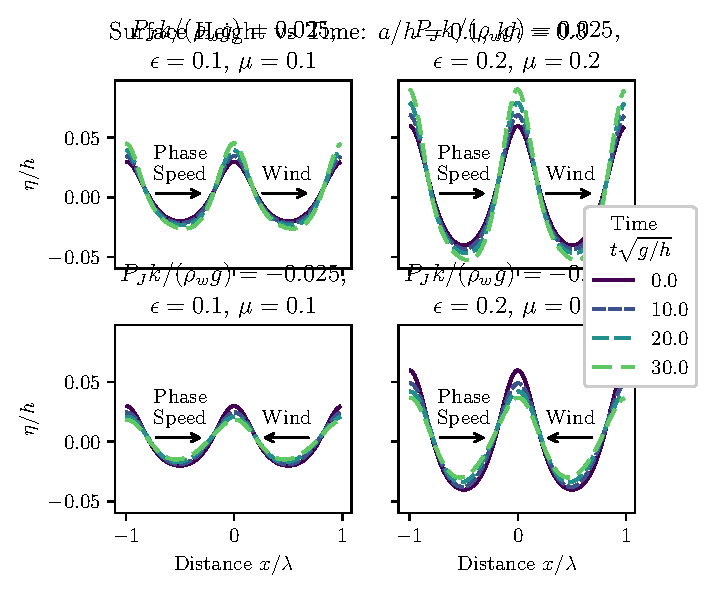
\includegraphics{Snapshots-Positive-Negative-Cnoidal.eps}
  \caption{
    Evolution of cnoidal profile under onshore and offshore Jeffreys
    forcing.
  }
\end{figure}

\begin{figure}
  \centering
  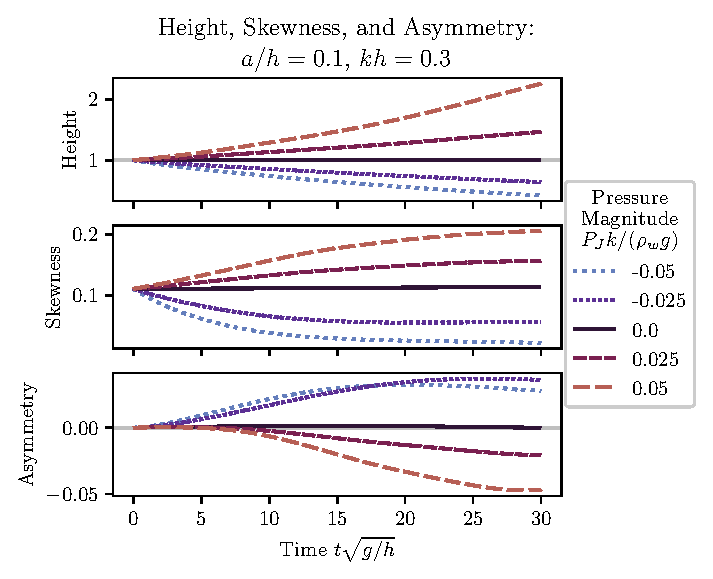
\includegraphics{Skew-Asymm-Cnoidal.eps}
  \caption{
    Skewness and asymmetry of cnoidal profile under onshore and offshore
    Jeffreys forcing.
  }
\end{figure}

\subsection{Generalized Miles Forcing}

\begin{figure}
  \centering
  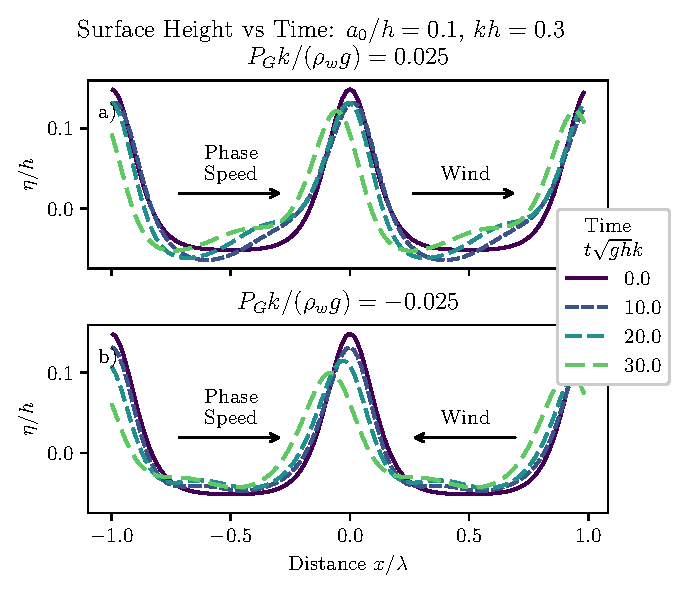
\includegraphics{Snapshots-Positive-Negative-Cnoidal-GM.eps}
  \caption{
    Evolution of cnoidal profile under onshore and offshore Generalized
    Miles forcing.
  }
\end{figure}

\begin{figure}
  \centering
  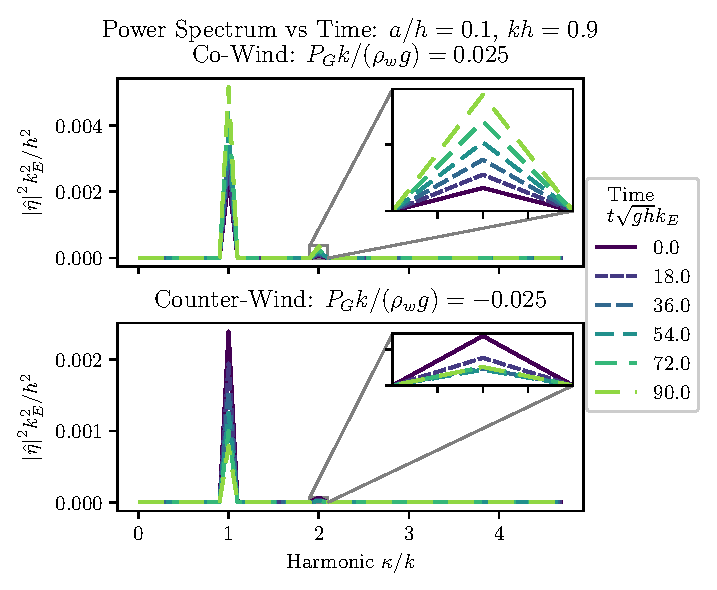
\includegraphics{Power-Spectrum-GM.eps}
  \caption{
    Power spectrum of cnoidal wave under Generalized Miles forcing.
  }
\end{figure}

It appears to preferentially enhance the higher harmonics, which can be
seen by looking at the power spectrum $\abs{\hat{\eta}}^2$ as a function
of time.
In particular, when the wind is blowing \emph{against} the wave, the
second harmonic is \emph{enhanced}, whereas we expect all harmonics to
be suppressed.
Also, this seems to be more pronounced for large $\psi_P$, like $\psi_P
= 3\pi/4$, whereas small $\psi_P \ll 1$ show the expected behaviour.
This leads to the growth of the second harmonic large relative to the
primary, essentially bifurcating the crest.
Therefore, the Generalized Miles type forcing seems unrealistic.

This is not surprising.
If we temporarily include the pressure at leading order for simplicity,
the leading order equations become
\begin{gather}
  \pdv{\eta_0}{t_0} + \pdv[2]{\varphi_0}{x} = 0 \,, \\
  \eta_0 + \pdv{\varphi_0}{t_0} = -p_0 \,.
\end{gather}
Eliminating $\phi_0$ from this gives
\begin{equation}
  \pqty{\pdv[2]{t_0} - \pdv[2]{x} } \eta_0 = \pdv[2]{x} p_0 \,.
\end{equation}
Fourier transforming from $x$ to $m$ gives
\begin{equation}
  \pqty{\pdv[2]{t_0} + m^2 } \hat{\eta}_{0,m} = -m^2 \GenP
  \hat{\eta}_{0,m} \,.
\end{equation}
This gives
\begin{equation}
  \eta_0 \propto e^{\im(m x - \omega_m t_0)}
\end{equation}
with
\begin{equation}
  \omega_m = mk \sqrt{gh \pqty{1 + k \GenP}}
\end{equation}
where we have redimensionalized.
Then, the imaginary part of $\omega_m$ is
\begin{equation}
  \Im{\omega_m} = mk \sgn \pqty{\Im{\GenP}} \sqrt{\frac{gh}{2}} \sqrt{-1
    - k\Re{\GenP} + \sqrt{1 + k^2 \abs{\GenP}^2 + 2 k \Re{\GenP}}} .
\end{equation}
Crucially, notice that $\sgn[\Im{\omega_m}] = \sgn{\Im{\GenP}}$.
Therefore, if $\Im{\GenP}>0$, mode-$m$ grows; if $\Im{\GenP} <
0$, mode-$m$ shrinks.

First, consider the Jeffreys case, where $\GenP = \pm \im m P$.
For the co-wind case, the $(+)$ sign is chosen and $\Im{\GenP} > 0$ for
all modes, causing each harmonic to grow.
For the counter-wind case, the $(-)$ sign is chosen and $\Im{\GenP} < 0$
for all modes, causing each harmonic to shrink.
This is the expected behavior.

Consider now Generalized Miles, where $\GenP = P \exp(\im m \psi_P)$.
The plots are made for $\psi_P = \pm 3\pi/4$ (positive for
co-wind, negative for counter-wind).
For the co-wind case, $\Im{\POne} = P \cos(3\pi/4) > 0$ and the primary
grows, while $\Im{\PTwo} = P \cos(3\pi/2) = -P$ and the first harmonic
shrinks quickly.
Technically, the $m=6$ mode grows quicker than the primary (since
$\Im{\hat{P}_6} = P \cos(9\pi/2) = P$), but since it is so much smaller
than the primary, it takes a long time to become noticeable.

However, for the counter-wind case $\Im{\POne} = P \cos(-3\pi/4) < 0$ and the primary
shrinks, while $\Im{\PTwo} = P \cos(-3\pi/2) = P$ and the first harmonic
\emph{grows} quickly.
Thus, within a relatively short time, the first harmonic becomes
dominant.
Thus, GM is a poor choice.

\appendix

\section{Energy Growth Rate \label{sec:energy_growth_rate}}
As a useful check on our earlier estimation of the magnitude of $P'$, we
can derive the energy growth rate.
Multiplying \cref{eq:kdv_burgers} by $\eta_0$, we find
\begin{equation}
  \frac{1}{2} \pdv{t_1} \eta_0^2 + P_J \frac{1}{4} (\eta_0^2)'' -
  \frac{1}{2} P_J (\eta_0')^2 + \frac{1}{2} (\eta_0^3)' + \frac{1}{12}
  (\eta_0^2)''' - \frac{1}{4} \bqty{\pqty{\eta_0'}^2}' = 0 \,.
\end{equation}
Then, integrating over a wavelength gives
\begin{equation}
  \begin{split}
  \pdv{t_1} \int_{-L/2}^{L/2} \frac{1}{2} \eta_0^2 \dd{x} &=
  \int_{-L/2}^{L/2} \frac{1}{2} P_J (\eta_0')^2 \dd{x}
  + \int_{-L/2}^{L/2} -P_J \frac{1}{4} (\eta_0^2)''  - \frac{1}{2} (\eta_0^3)' - \frac{1}{12}
  (\eta_0^2)''' + \frac{1}{4} \bqty{\pqty{\eta_0'}^2}' \dd{x}
  \\
  &=
  \int_{-L/2}^{L/2} \frac{1}{2} P_J (\eta_0')^2 \dd{x}
  + \eval{\bqty{-P_J \frac{1}{4} (\eta_0^2)'  - \frac{1}{2} (\eta_0^3) - \frac{1}{12}
  (\eta_0^2)'' + \frac{1}{4} \pqty{\eta_0'}^2}}_{-L/2}^{L/2}
  \\
  &=
  \int_{-L/2}^{L/2} \frac{1}{2} P_J (\eta_0')^2 \dd{x}
   \,.
  \end{split}
\end{equation}
Redimensionalizing, we find
\begin{equation}
  \frac{k}{\rho_w a^2} \frac{1}{\omega_0 \epsilon} \pdv{t} \int_{-L/2}^{L/2}
  \rho_w \eta^2 \dd{x} = \frac{1}{k a^2} \int_{-L/2}^{L/2} P_J'
  (\partial_x \eta)^2 \dd{x}
\end{equation}
or
\begin{equation}
  \frac{1}{\omega_0 E} \pdv{t} E =
  \epsilon
  \frac{
    \int_{-L/2}^{L/2} P_J' (\partial_x \eta)^2 \dd{x}
  }
  {
    \int_{-L/2}^{L/2} k^2 \eta^2 \dd{x}
  }
\end{equation}
with $E = \rho_w \int_{-L/2}^{L/2} \eta^2 \dd{x}$ the average
energy per wavelength.
The left-hand side is simply $\gamma/\omega_0$.
If, for simplicity, we consider a simple sinusoid $\eta_0 = A \cos(k x -
\omega_0 t)$, we find
\begin{equation}
  \frac{\gamma}{\omega_0} = \epsilon P_J' = \frac{P_J k}{\rho_w g} \,,
\end{equation}
where we used $\alpha = \epsilon$.

\printbibliography{}

\end{document}
